\chapter{Background}
\label{back}

In this section we talk about all background knowledge necessary to 

\section{Da Vinci Surgical System}
\label{sec:daVinci}

Da Vinci is the first FDA approved surgical robotic system. It can be used for various types of surgeries such as cardiac, colorectal, thoracic, urological and gynecologic. More than 3 million operation were performed worldwide using da Vinci system. \cite{_intuitive_2018}

Effectiveness of da Vinci system in comparison to opened surgery and other systems \cite{yu_safety_2014}

\section{Current Approaches}
\label{sec:CurAppr}

Placing force sensors on the surgical instrument \cite{hong_design_2012}

Making new surgical instrument design \cite{schwalb_forcesensing_2017}

Vision based solution \cite{aviles_towards_2017}

measuring the proximal guide wire force \cite{yoon_design_2015}

Senhance robot with force feedback, which is FDA approved. Principle - put 6-DOF force sensor 


\section{Force sensors}
\label{sec:ForceSensors}

Two general principles dominate in force measurement: piezoelectric and strain-gauge sensors. \cite{SGandP1}

Piezoelectric sensors consist of two crystal disks with an electrode foil in between. When force is applied, an electric charge, proportional to the applied force, is obtained and can be measured. Piezoelectric sensors show small deformation when force is applied, this results in a high resonance frequency. Also, piezoelectric sensors due to their principle of operation have significant linearity error and drift. \cite{SGandP2}

In the strain gauge based force transducers the force causes deformation and subsequent linear change in resistance. Strain gauges are usually connected to a Wheatstone bridge circuit, where the output voltage is proportional to the applied force. Strain gauge based transducers provide small individual errors (200 ppm), show no drift, and are therefore appropriate for long-term monitoring tasks. However, they are relatively big, temperature dependent, and have lower resonance frequency in comparison to piezoelectric sensors. \cite{SGandP1,SGandP2}

On the basis of the above mentioned, piezoelectric sensors are preferable for dynamic measurements of small forces while strain gauge sensors are better when large forces are measured. In this study, strain gauges were used since they show better accuracy and long-term stability. \cite{SGandP1,SGandP2}

We can use QTC-pills, but it has no-linearity and hysteresis issues. We can test in the future.


\section{Literature Review}
\label{sec:LitRev}

Write about all disadvantages of previous methods.

Tools - >limited lifetime - find citation

Vision -> huge time delays, accuracy

Wire force - > repeatability issue

Write about my approach
Trying to put sensors on the shaft itself, on the cannula, on the sleeve to see where we get the most sensitive results

Here is a figure: Fig.\ref{fig:exampleFigure} and here is a table: Table \ref{tab:Protocol}.

\begin{figure}[h]
  \begin{center}
    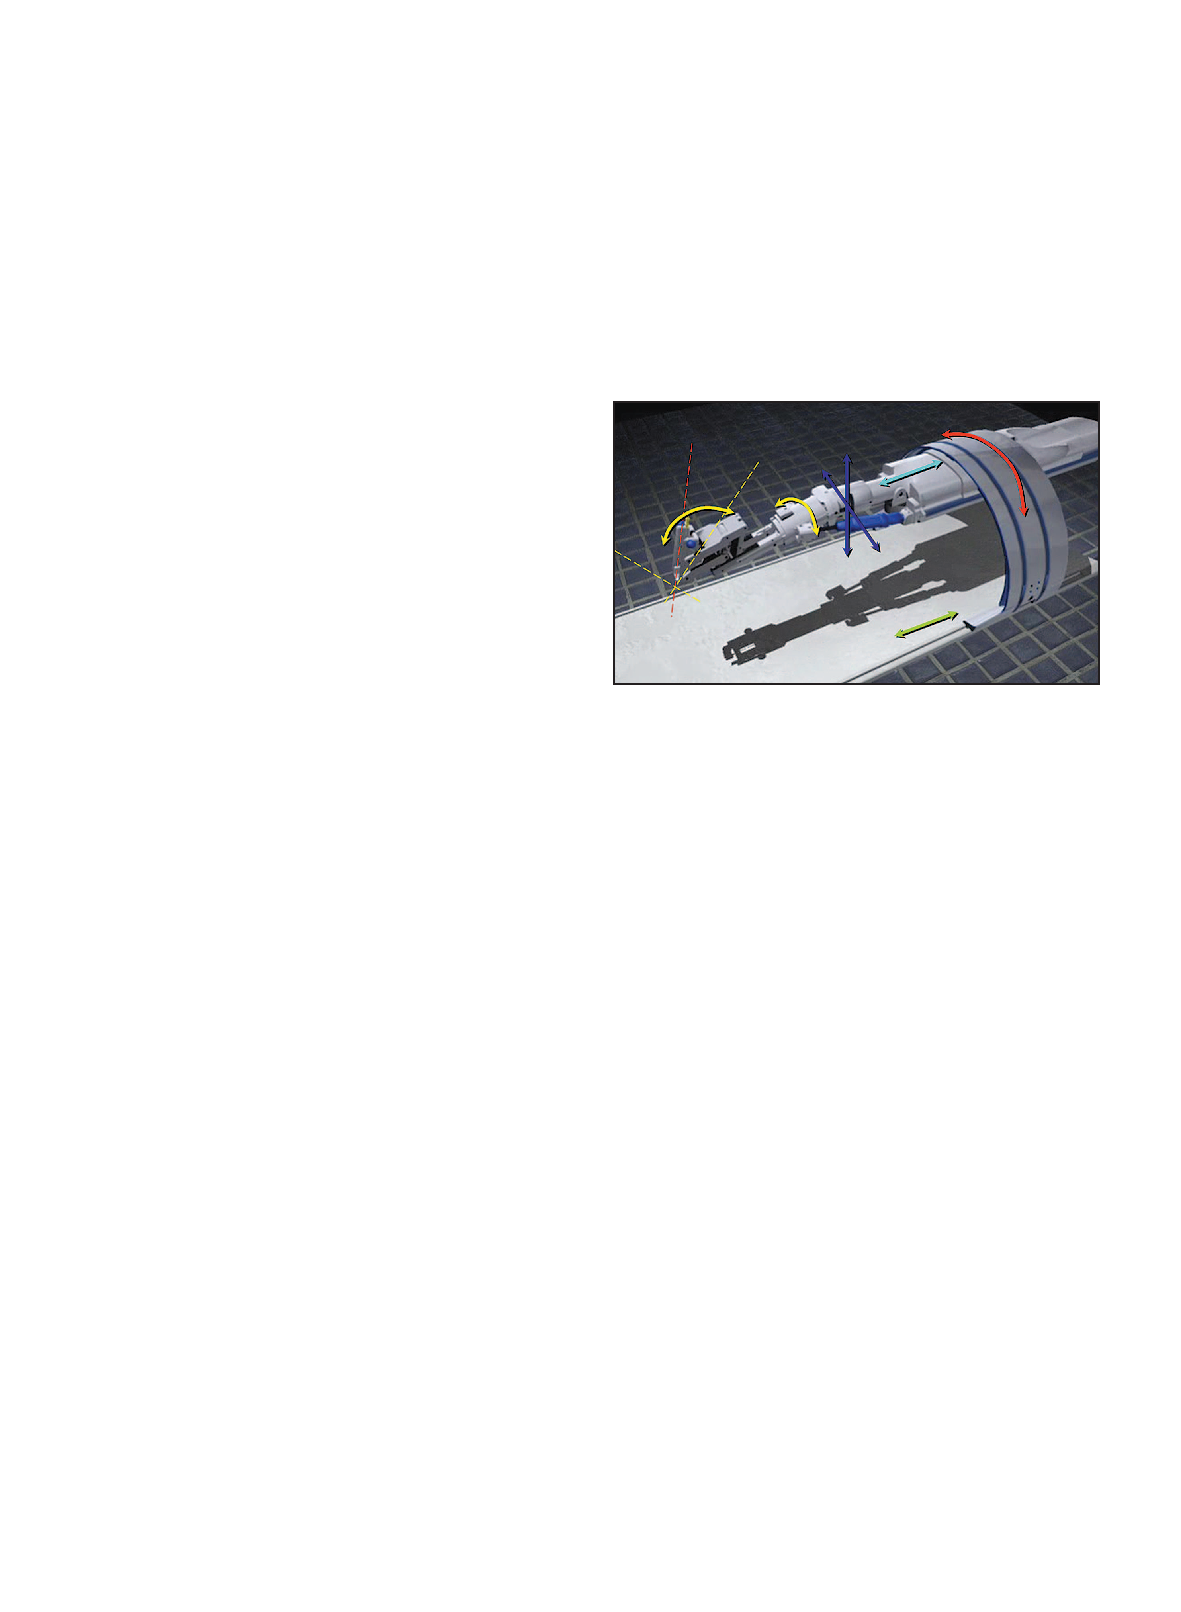
\includegraphics[width=120mm]{Fig/chap1/innomotion.pdf}
  \end{center}
  \vspace{-4mm}
\caption[CAD model of the Innomotion robotic system.]
{This is a sample figure with a sample citation \cite{Fischer2008_TMECH} \copyright 2008 IEEE.}
 \label{fig:exampleFigure}
\vspace{-2mm}
\end{figure}

\begin{table}[htb]
  \begin{center}
\caption[Scan parameters for compatibility evaluation.]{Detailed scan parameters for each of four protocols for compatibility evaluation}
\label{tab:Protocol}
  \end{center}
\includegraphics[width=150mm]{Fig/chap1/Protocol.pdf}
%\caption*{}
\end{table}
\vspace{-2mm}

\section{My approach}
\label{sec:MyAppr}
Trying to put sensors on the shaft itself, on the cannula, on the sleeve to see where we get the most sensitive results

\subsection{Requirements for the device}
\label{sec:DevReq}
Biocompatibility

Linearity

Range of forces 
Highest gripping force in Da Vinci tool was seen in the Hemo-lok[R] clip applier (39.92 [+ or -] 0.89 N).
0.3 - 11 N. 
Tensile strength and failure load of sutures for robotic surgery
Others

\subsection{Strain gauge}
\label{sec:SGReq}
According to the manual for strain gauge selection provided by Vishay Micro-Measurements. The strain gauge should have following parameters:
• Gauge length is 0.8 mm. Ideally gauge length should be 10 \% of the shaft radius;
• Single grid;
• Isoelastic (D alloy) that has higher gauge factor with E backing;
• Encapsulated with pre attached leads;
• Resistance – 120 Ohms;
• Gauge factor - 2;
• STC – number (self-temperature-compensation): DY – dynamic
Since the diameter of the shaft is only 8.5 mm, one of the most important parameters, in this
case, is the size of the strain gauge. Another important parameter is gauge‘s resistance, sensitivity
of the strain gauge drastically depends on this parameter. Strain gauges with different resistivity
were used (350 and 120 Ohms and sizes of 6 x 2.5 mm).

\subsection{Sleeve designs}
\label{sec:SlevDes}
We designed different sleeves to get..

\subsection{Sensor Location}
\label{sec:SenLoc}
Sensor location on sleeves, shaft and cannula - include COMSOL studies
Strain Gauge Placement
A qualitative analysis was done in Solidworks to assess better placement of the strain gauges on the shaft or cannula. First we found elasticity modulus of the shaft and cannula, and used them for further analysis.


